\section{Methodology}
\label{sec:methodology}

\begin{figure}[!t]
\centering
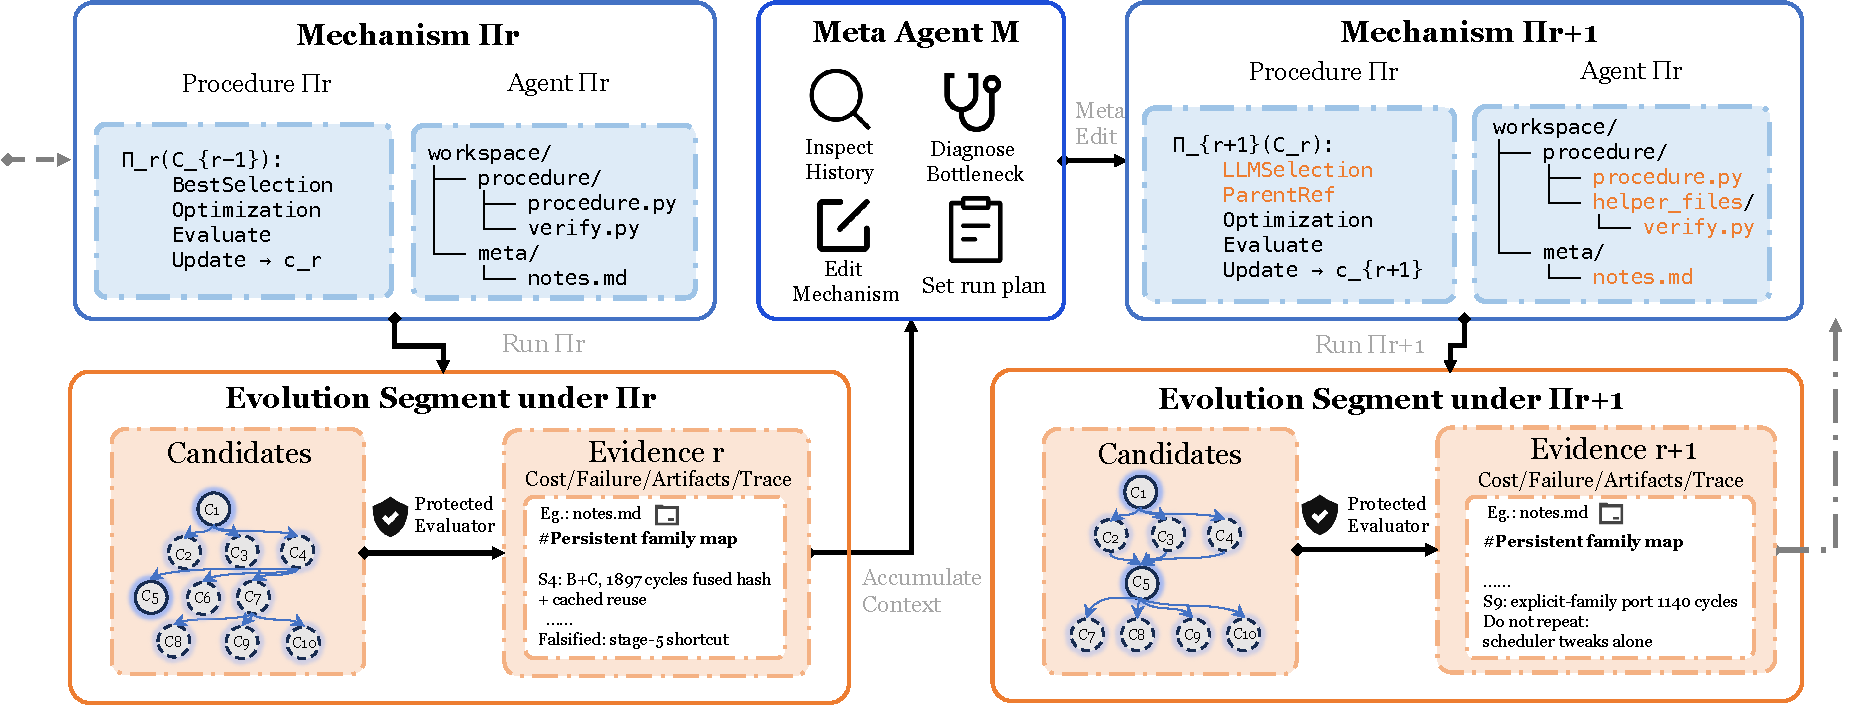
\includegraphics[width=\linewidth]{images/Figure-2.pdf}
\caption{
\textbf{Architecture of \method.}
The harness runs evolution segments under the current mechanism $\Pi_r$, protects evaluation, and records structured evidence.
A meta-agent observes this evidence to edit $\Pi_r$ into $\Pi_{r+1}$ and set the next run plan, enabling coarse-grained intervention over both procedures and agent contexts.
}
\label{fig:main_figure}
\end{figure}

Figure~\ref{fig:main_figure} illustrates \method.
\method instantiates the environment view in Section~\ref{sec:formulation} as a harnessed loop that alternates between a \emph{meta-editing phase} and an \emph{evolution segment}.
In the meta-editing phase, the meta-agent updates the current evolution mechanism $\Pi_r$ and specifies how the next segment should run, including its iteration budget and stopping conditions.
In the evolution segment, the updated mechanism runs under this plan and may produce multiple evaluated candidates before the next meta-agent intervention.
Thus, one meta-edit can govern a segment of future evolution rather than a single candidate.

\subsection{Design of \method}
\label{sec:design}

\textbf{Meta-editing phase.}
The meta-editing phase decides both \textbf{what to change} and \textbf{how to continue}.
The meta-agent can be any coding-capable agent that can inspect a workspace, edit files, execute commands, and follow the \method meta-agent skill specification, such as Claude Code~\citep{claudecode2025}, Codex~\citep{codex2025}, or open-source coding agents~\citep{yang2024sweagent, opencode2025}.
Given the current workspace, it inspects the accumulated history, then produces a meta-action consisting of a workspace edit and a run plan.
The workspace edit modifies files that define $\Pi_r$, such as procedure code, prompts, skills, goals, tools, feedback formats, validators, notes, or execution context.
The run plan specifies how the next evolution segment should proceed, including the allowed iterations, budget use, and stopping conditions.

This design makes the meta-agent a process-level editor rather than a candidate generator: it changes the mechanism and conditions under which future candidates are produced.
When evolution is productive, the meta-agent may allocate more iterations to the current mechanism; when it repeatedly produces invalid candidates, redundant attempts, or irrelevant exploration, the meta-agent may stop the segment and revise $\Pi_r$ before continuing.
The full meta-agent skill specification and pseudocode of the meta-editing loop are provided in Appendix~\ref{app:meta_agent_skill}.

\textbf{Harnessed evolution segment.}
An evolution segment is the interval executed after a meta-edit.
It runs the current mechanism $\Pi_r$ under the run plan produced by the meta-agent.
Depending on the setting, this segment may consist of several rounds of a procedure, or an inner-agent session that produces multiple candidate attempts.
Each candidate submitted for official evaluation passes through the harness-controlled evaluator, and the resulting artifact, score, trace, failure information, cost, and provenance are appended to the candidate history.

The harness provides the stable boundary needed for reliable meta-editing.
It organizes candidates, logs, traces, evaluation records, meta-agent instructions, and editable evolution components into a fixed workspace layout.
To prevent reward hacking, the evaluator is isolated from both the evolution agent and the meta-agent: agents can submit candidates, but they cannot inspect evaluator internals, access hidden benchmark artifacts, or directly write official scores.
The harness further exposes a command-line interface for initializing workspaces, launching evolution segments, inspecting recent status and candidate history, and continuing the current process.
Thus, the harness does not decide how evolution should improve; it provides the protected and inspectable interface through which evolution can be observed, edited by the meta-agent, recorded, and resumed.

\subsection{Instantiating \method}
\label{sec:instantiation}

\method applies the same two-phase loop to both forms of agentic evolution.
The outer loop is unchanged: the meta-agent edits the current mechanism $\Pi_r$ and specifies how the next evolution segment should run.
The difference lies in what $\Pi_r$ consists of.

\textbf{Procedure-based evolution.}
For procedure-based evolution, $\Pi_r$ is an explicit evolution procedure.
It defines how previous candidates or contexts are selected, how new candidates are generated, how evaluation feedback is used, and how candidate history is updated.
A meta-action therefore edits the procedure itself, such as revising the selection strategy, changing the optimization operator, altering the feedback summary, adding local filtering or retry logic, adjusting budget use, or repairing candidate management.
The edited procedure then controls the next evolution segment, which may run for multiple rounds before the next meta-agent intervention.

\textbf{Agent-based evolution.}
For agent-based evolution, $\Pi_r$ is the operating context of a general-purpose evolution agent, including goals, skills, tools, memory files, shared notes, validators, and execution setup.
A meta-action therefore edits the conditions under which the next inner-agent session will evolve, such as revising a skill, rewriting the session goal, changing how evaluator feedback is presented, or reorganizing shared notes.
The inner agent remains responsible for generating candidates, while \method revises the context that shapes future evolution.